\chapter{Conception}

\section*{Introduction}

Ce chapitre traduit les besoins du chapitre précédent en une
\textbf{architecture technique} précise. Il présente d'abord
l'architecture globale du système, puis l'infrastructure AWS et
l'architecture Docker, le modèle de données, plusieurs scénarios
d'interaction (diagrammes de séquence) et enfin la conception de la
sécurité \textbf{en profondeur}.

\section{Architecture globale}

L'architecture cible peut être résumée par la figure
\ref{fig:archi-globale}. Le navigateur du client résout d'abord le
nom de domaine \texttt{webcyber.app} via Route\,53, qui retourne
l'\textbf{Elastic IP} de l'instance EC2. La requête HTTPS atteint
ensuite l'instance, où elle traverse le \textbf{Security Group} avant
d'être servie par le conteneur Nginx, qui terminera TLS et
\emph{proxifiera} la requête vers l'application Flask.

\begin{figure}[H]
  \centering
  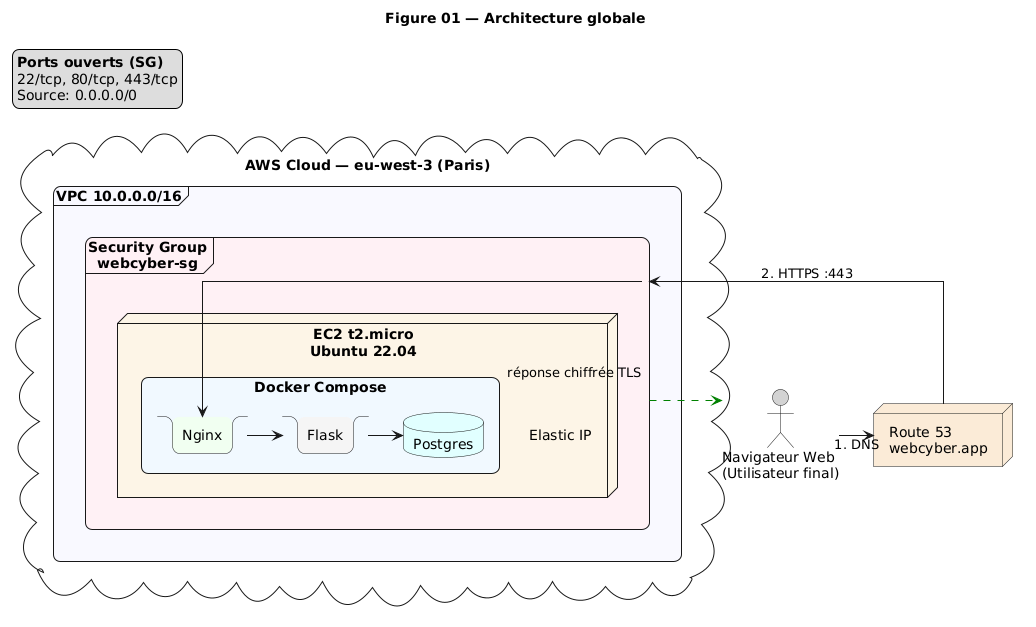
\includegraphics[width=\linewidth]{figures/img/fig01-architecture-globale.png}
  \caption{Architecture globale --- vue d'ensemble.}
  \label{fig:archi-globale}
\end{figure}

\subsection{Composants et responsabilités}

\begin{longtable}{P{3cm} P{11cm}}
\toprule
\textbf{Composant} & \textbf{Responsabilité} \\
\midrule
\endhead
Route\,53        & Résolution DNS : \texttt{webcyber.app} \(\to\) Elastic IP. \\
Elastic IP       & Adresse IPv4 publique fixe associée à l'EC2. \\
EC2 (t2.micro)   & Hôte Ubuntu 22.04 exécutant Docker. \\
Security Group   & Pare-feu \emph{stateful} au niveau de l'EC2. \\
Conteneur Nginx  & Proxy inverse, terminaison TLS, en-têtes de sécurité. \\
Conteneur Flask  & Logique applicative, authentification, CRUD. \\
Conteneur PostgreSQL & Persistance des données utilisateur. \\
\bottomrule
\end{longtable}

\section{Infrastructure AWS}

\subsection{Choix de la région}

La région \texttt{eu-west-3} (Paris) a été choisie pour sa proximité
géographique (latence réduite vers la Mauritanie et l'Europe
francophone) et pour des considérations de \emph{résidence des données}
(stockage en Europe).

\subsection{Composants AWS retenus}

La figure \ref{fig:aws-infra} détaille l'organisation interne au
\emph{cloud}. Les choix retenus privilégient la \textbf{simplicité} et
la \textbf{lisibilité} pédagogique :

\begin{itemize}
  \item utilisation du \textbf{VPC par défaut} (CIDR
        \texttt{172.31.0.0/16}) sans VPC personnalisé;
  \item un \textbf{sous-réseau public} unique;
  \item un \textbf{Security Group dédié} (\texttt{webcyber-sg});
  \item une seule \textbf{instance EC2} \texttt{t2.micro};
  \item une \textbf{Elastic IP} associée;
  \item une \textbf{zone hébergée Route\,53} pour le domaine
        \texttt{webcyber.app}.
\end{itemize}

\begin{figure}[H]
  \centering
  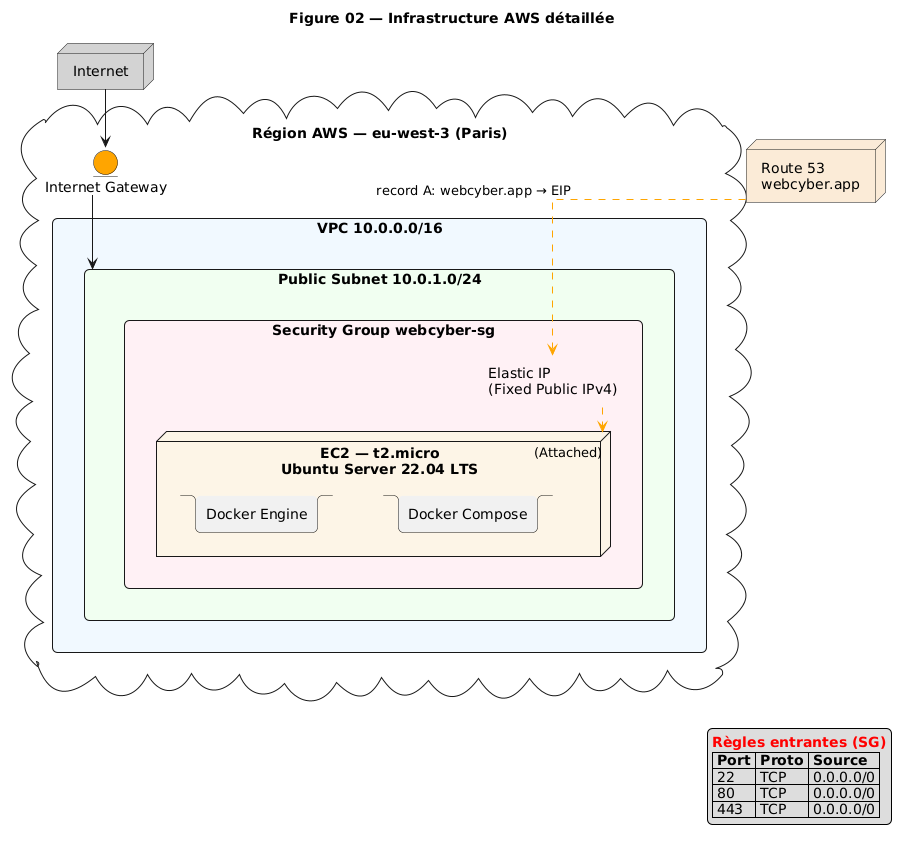
\includegraphics[width=\linewidth]{figures/img/fig02-aws-infrastructure.png}
  \caption{Infrastructure AWS détaillée.}
  \label{fig:aws-infra}
\end{figure}

\subsection{Règles du Security Group}

Le pare-feu réseau du périmètre est un \textbf{Security Group}
\emph{stateful} : seul le trafic entrant explicitement autorisé est
accepté, et les réponses correspondantes sont automatiquement
autorisées en sortie.

\begin{table}[H]
\centering
\caption{Règles entrantes du Security Group \texttt{webcyber-sg}.}
\begin{tabular}{C{2cm} C{2cm} C{1.5cm} P{4cm} P{4cm}}
\toprule
\textbf{Type} & \textbf{Protocole} & \textbf{Port} & \textbf{Source} & \textbf{Justification} \\
\midrule
SSH   & TCP & 22  & \texttt{0.0.0.0/0} & Administration distante \\
HTTP  & TCP & 80  & \texttt{0.0.0.0/0} & Redirection vers HTTPS \\
HTTPS & TCP & 443 & \texttt{0.0.0.0/0} & Trafic web chiffré \\
\bottomrule
\end{tabular}
\end{table}

Aucun autre port n'est ouvert. Les ports applicatifs (\texttt{5000}
pour Flask, \texttt{5432} pour PostgreSQL) restent confinés au réseau
Docker interne et ne sont donc pas accessibles depuis Internet.

\subsection{Estimation des coûts}

\begin{table}[H]
\centering
\caption{Estimation mensuelle (sous \emph{free tier} AWS).}
\begin{tabular}{P{6cm} R{3cm}}
\toprule
\textbf{Ressource} & \textbf{Coût} \\
\midrule
EC2 \texttt{t2.micro}            & \$0,00 \\
EBS 20~Gio gp3                   & \$0,00 \\
Elastic IP (associée)            & \$0,00 \\
Route\,53 zone hébergée          & \$0,50 \\
Trafic sortant (faible)          & $\approx$ \$0,00 \\
\midrule
\textbf{Total estimé}            & $\approx$ \textbf{\$0,50/mois} \\
\bottomrule
\end{tabular}
\end{table}

\section{Architecture Docker}

\subsection{Vue d'ensemble}

Trois conteneurs cohabitent sur l'instance, orchestrés par Docker
Compose et reliés par un réseau \emph{bridge} privé
(\texttt{webcyber-net}). La figure \ref{fig:docker-archi} montre cette
organisation, ainsi que les volumes persistants utilisés.

\begin{figure}[H]
  \centering
  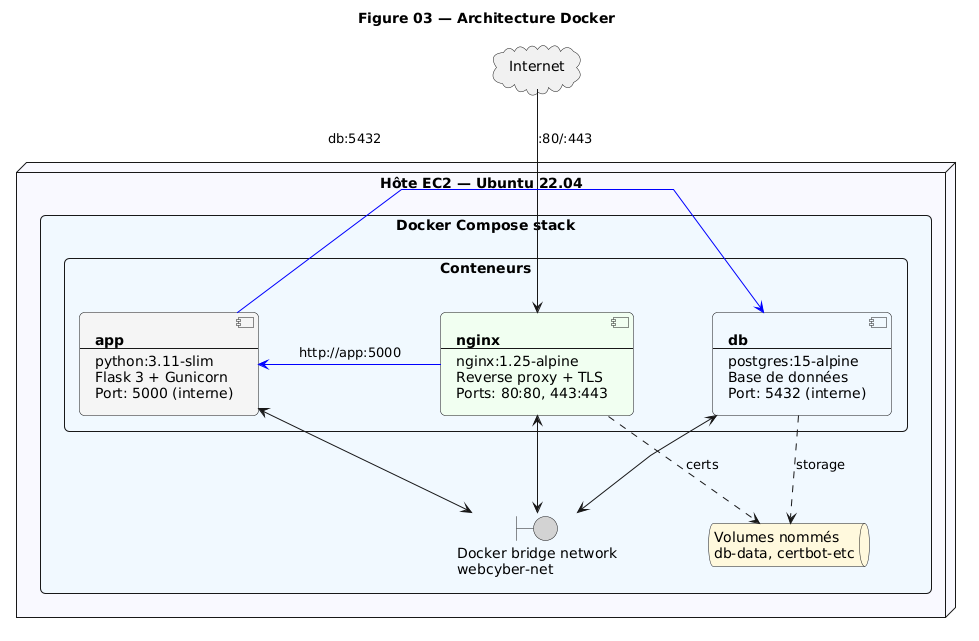
\includegraphics[width=\linewidth]{figures/img/fig03-docker-architecture.png}
  \caption{Architecture Docker --- trois conteneurs sur réseau \emph{bridge}.}
  \label{fig:docker-archi}
\end{figure}

\subsection{Spécifications des conteneurs}

\begin{longtable}{P{2cm} P{5cm} P{2.5cm} P{4cm}}
\toprule
\textbf{Service} & \textbf{Image} & \textbf{Ports} & \textbf{Rôle} \\
\midrule
\endhead
\texttt{nginx} & \texttt{nginx:1.25-alpine} & 80, 443 (publiés) & Proxy inverse, TLS, en-têtes de sécurité \\
\texttt{app}   & \texttt{python:3.11-slim} (build) & 5000 (interne) & Application Flask + Gunicorn \\
\texttt{db}    & \texttt{postgres:15-alpine} & 5432 (interne) & Base de données PostgreSQL \\
\bottomrule
\end{longtable}

Le \emph{principe d'exposition minimale} est appliqué : seul le proxy
publie ses ports vers l'hôte. Les services \texttt{app} et \texttt{db}
ne sont accessibles qu'\emph{intra-Docker}, par leur nom de service
(résolution DNS embarquée par Docker).

\subsection{Volumes persistants}

\begin{itemize}
  \item \texttt{db-data} : données PostgreSQL (table \texttt{users},
        table \texttt{notes}, indexes, WAL).
  \item \texttt{certbot-etc} : certificats Let's Encrypt et clés
        privées.
  \item \texttt{certbot-var} : état interne de Certbot (compte ACME,
        \emph{lock files}).
\end{itemize}

\subsection{Estimation des ressources}

Sur \texttt{t2.micro} (1~Gio RAM), l'occupation mémoire prévisionnelle
est confortable :

\begin{table}[H]
\centering
\caption{Empreinte mémoire estimée des conteneurs.}
\begin{tabular}{P{4cm} R{4cm}}
\toprule
\textbf{Conteneur}   & \textbf{Mémoire estimée} \\
\midrule
Nginx                & 10--30 Mio \\
Flask + 2 \emph{workers} Gunicorn & 100--200 Mio \\
PostgreSQL           & 50--100 Mio \\
Surcharge Docker     & $\approx$ 100 Mio \\
\midrule
\textbf{Total}       & $\approx$ \textbf{300--430 Mio} \\
\bottomrule
\end{tabular}
\end{table}

\section{Modèle de données}

Le modèle de données est volontairement réduit à deux entités, comme
le montre la figure \ref{fig:classes}.

\begin{figure}[H]
  \centering
  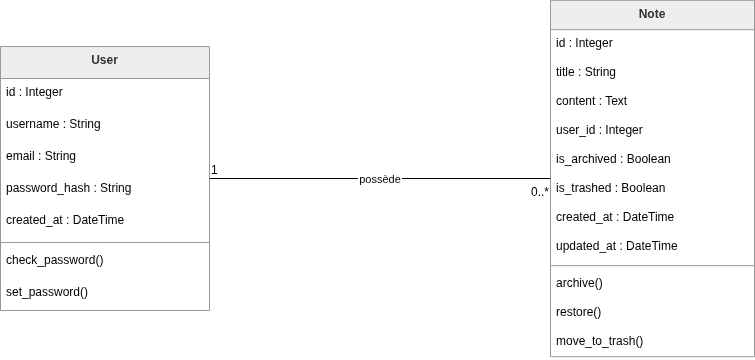
\includegraphics[width=0.95\linewidth]{figures/img/fig05-diagramme-classes.png}
  \caption{Diagramme de classes (modèle de données).}
  \label{fig:classes}
\end{figure}

\subsection{Description}

\begin{itemize}
  \item Un \textbf{User} possède de zéro à $n$ \textbf{Notes}.
  \item Une \textbf{Note} appartient à exactement un \textbf{User}, via
        la clé étrangère \texttt{user\_id}.
  \item Les drapeaux \texttt{is\_archived} et \texttt{is\_trashed}
        permettent une suppression \emph{douce} (corbeille) et une
        archive sans déplacer ni dupliquer la donnée.
\end{itemize}

\subsection{Considérations de sécurité dans le modèle}

\begin{itemize}
  \item Le champ \texttt{password\_hash} contient uniquement le
        \emph{hachage} du mot de passe, jamais sa valeur en clair.
  \item Les contraintes \texttt{UNIQUE} sur \texttt{username} et
        \texttt{email} préviennent les doublons et certaines attaques
        d'énumération.
  \item Toutes les requêtes \texttt{SELECT}, \texttt{UPDATE} ou
        \texttt{DELETE} sur la table \texttt{notes} \textbf{doivent}
        comporter le filtre \texttt{WHERE user\_id = current\_user.id}.
\end{itemize}

\section{Diagrammes de séquence}

\subsection{Authentification}

Le scénario d'authentification met en jeu cinq acteurs : l'utilisateur,
son navigateur, Nginx, Flask et PostgreSQL. La figure
\ref{fig:seq-auth} en détaille le déroulement, depuis la saisie des
identifiants jusqu'à la création de la session côté serveur et au
positionnement du \emph{cookie} dans le navigateur.

\begin{figure}[H]
  \centering
  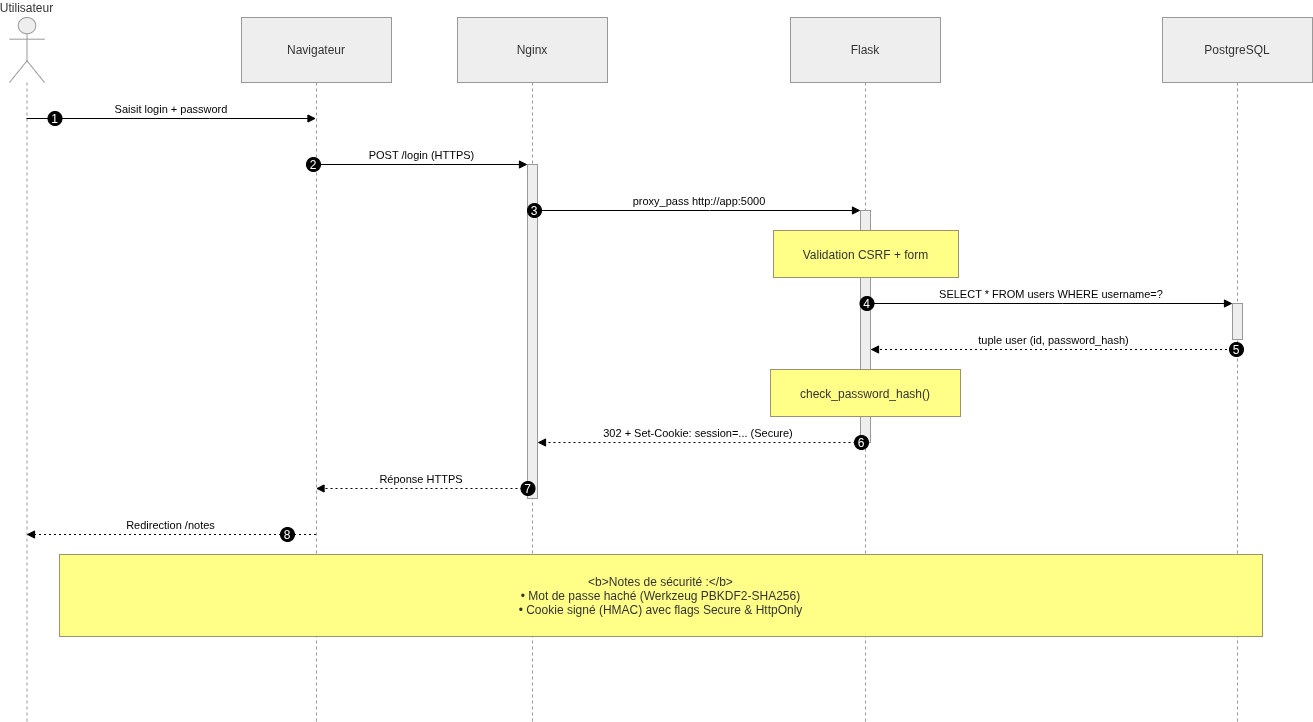
\includegraphics[width=\linewidth]{figures/img/fig06-sequence-authentification.png}
  \caption{Diagramme de séquence --- authentification.}
  \label{fig:seq-auth}
\end{figure}

Trois éléments de sécurité sont à noter :

\begin{enumerate}
  \item le mot de passe ne quitte jamais le tunnel TLS;
  \item la comparaison côté serveur passe par
        \texttt{check\_password\_hash}, qui exécute une comparaison
        \emph{constant-time};
  \item le \emph{cookie} de session est signé (HMAC), et porte les
        attributs \texttt{Secure}, \texttt{HttpOnly} et
        \texttt{SameSite=Lax}.
\end{enumerate}

\subsection{Création d'une note}

Le scénario de création d'une note (figure \ref{fig:seq-note}) montre
en particulier le contrôle de session
(\texttt{@login\_required}), la vérification du jeton CSRF, puis
l'insertion en base avec association à l'utilisateur courant.

\begin{figure}[H]
  \centering
  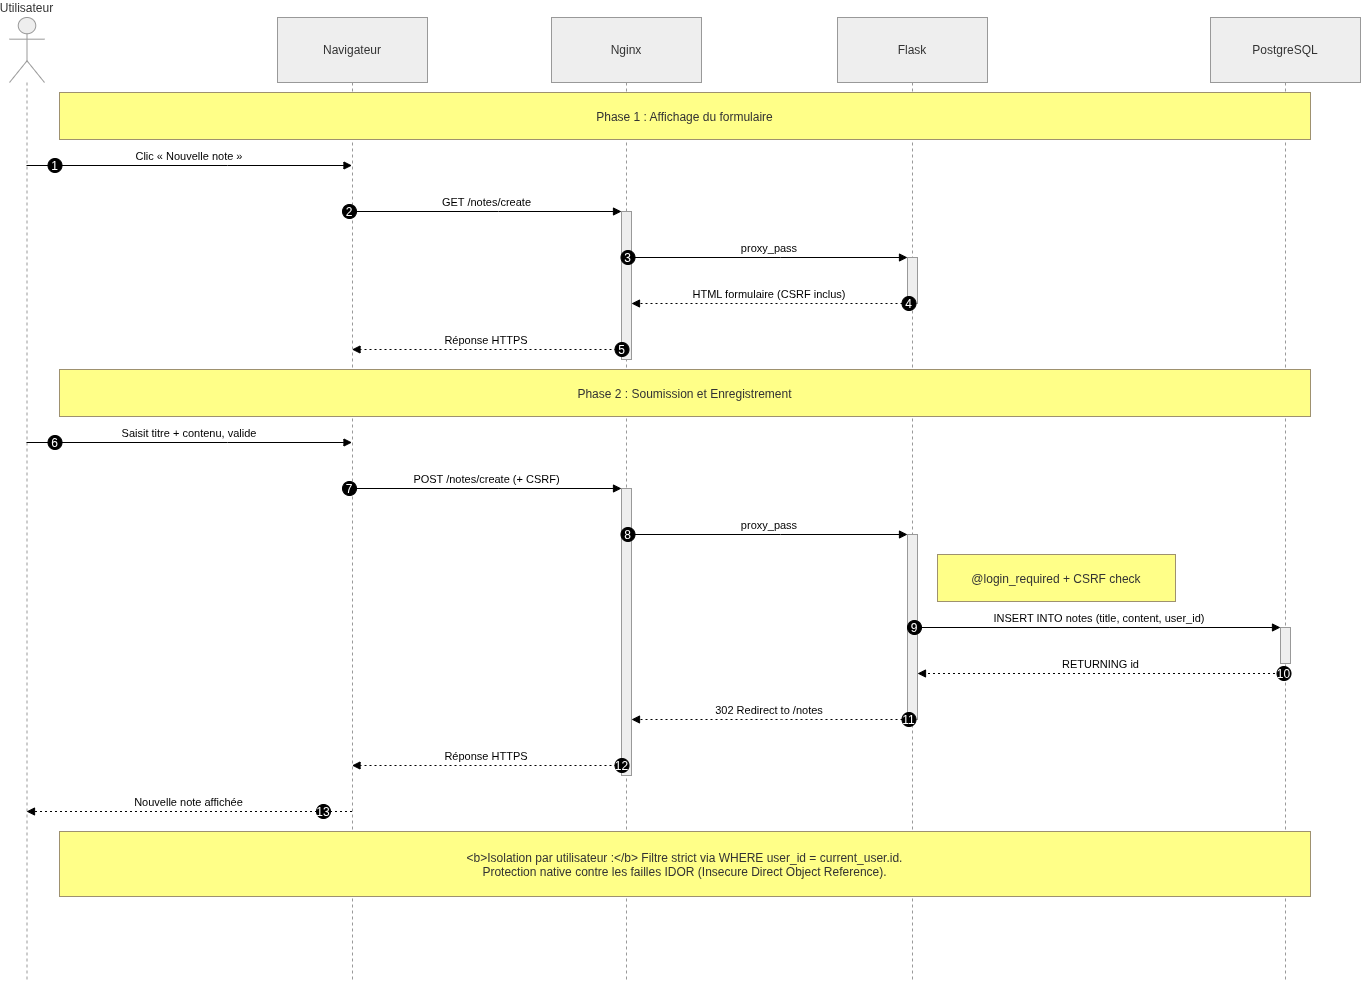
\includegraphics[width=\linewidth]{figures/img/fig07-sequence-note.png}
  \caption{Diagramme de séquence --- création d'une note.}
  \label{fig:seq-note}
\end{figure}

\section{Conception de la sécurité --- défense en profondeur}

La sécurité du système ne repose pas sur une unique mesure, mais sur
\textbf{six couches empilées}, chacune apportant une garantie
spécifique. La figure \ref{fig:couches-securite} en donne une
représentation synthétique.

\begin{figure}[H]
  \centering
  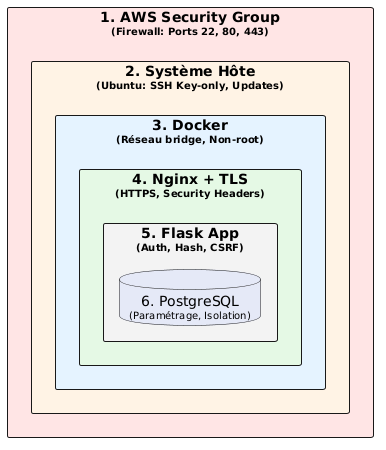
\includegraphics[width=\linewidth]{figures/img/fig09-couches-securite.png}
  \caption{Les six couches de sécurité (\emph{defense-in-depth}).}
  \label{fig:couches-securite}
\end{figure}

\subsection{Couche 1 --- Security Group}

Le Security Group AWS est un pare-feu \emph{stateful} qui constitue la
\textbf{première ligne de défense} : il bloque tout port non
explicitement autorisé. Sa configuration a été détaillée plus haut.

\subsection{Couche 2 --- Système hôte}

Sur l'instance EC2 :

\begin{itemize}
  \item \texttt{PermitRootLogin no} : interdiction du login SSH
        \texttt{root};
  \item authentification SSH par clé en mode primaire;
  \item \texttt{unattended-upgrades} pour appliquer les mises à jour
        de sécurité automatiquement;
  \item utilisateur applicatif \texttt{ubuntu} non-root.
\end{itemize}

\subsection{Couche 3 --- Isolation Docker}

\begin{itemize}
  \item Réseau \emph{bridge} privé \texttt{webcyber-net}; les
        conteneurs \texttt{app} et \texttt{db} ne publient pas de
        port;
  \item Le \emph{Dockerfile} de l'application crée un utilisateur
        non-privilégié \texttt{appuser} (UID 1000) et l'utilise pour
        l'exécution finale;
  \item Les volumes nommés isolent les données persistantes du système
        de fichiers de l'hôte.
\end{itemize}

\subsection{Couche 4 --- Nginx + TLS}

\begin{itemize}
  \item TLS 1.2 et 1.3 uniquement, profil \emph{Mozilla Intermediate};
  \item certificat \textbf{Let's Encrypt} renouvelé automatiquement;
  \item redirection \(80 \to 443\);
  \item en-têtes \textbf{HSTS}, \textbf{CSP}, \textbf{X-Frame-Options},
        \textbf{X-Content-Type-Options}, \textbf{Referrer-Policy}
        injectés sur toutes les réponses;
  \item \texttt{server\_tokens off} pour masquer la version de Nginx.
\end{itemize}

\subsection{Couche 5 --- Application Flask}

\begin{itemize}
  \item Hachage des mots de passe via
        \texttt{generate\_password\_hash} (PBKDF2-SHA256, sel
        automatique);
  \item Session signée par \texttt{SECRET\_KEY} aléatoire (32 octets);
  \item Protection \textbf{CSRF} sur tous les formulaires (Flask-WTF);
  \item Validation systématique des entrées par WTForms (longueur,
        type, présence);
  \item Décorateur \texttt{@login\_required} sur toutes les routes
        privées;
  \item Filtre \texttt{user\_id} sur 100\,\% des requêtes \emph{notes}.
\end{itemize}

\subsection{Couche 6 --- Base de données}

\begin{itemize}
  \item Utilisateur \texttt{webcyber\_user} non-superutilisateur;
  \item Mot de passe long et aléatoire (>=20 caractères) injecté via
        \texttt{.env};
  \item Pas de port publié vers l'hôte;
  \item Requêtes paramétrées par SQLAlchemy (pas de concaténation de
        chaînes SQL).
\end{itemize}

\section{Conclusion du chapitre}

La conception ainsi décrite est volontairement \emph{minimale mais
complète} : un seul serveur, trois conteneurs, deux entités, mais une
sécurité empilée sur six niveaux. Le chapitre suivant présente la
réalisation concrète de cette conception et les étapes de son
déploiement.
